
\chapter{Metodologia}
\label{chap:metodologia}

Esta pesquisa é classificada como \textbf{aplicada}, pois tem como finalidade gerar conhecimento direcionado à solução de um problema prático específico: a escolha de ferramentas de monitoramento adequadas para ambientes de virtualização de funções de rede \cite{gil2021}. Quanto à abordagem, é \textbf{quantitativa}, uma vez que os dados coletados são expressos numericamente e submetidos a tratamento estatístico \cite{marconi2017}. Em relação aos seus objetivos, caracteriza-se como \textbf{comparativa}, pois visa estabelecer diferenças e semelhanças de desempenho entre as três abordagens estudadas. Por fim, quanto ao procedimento técnico, trata-se de uma \textbf{pesquisa experimental}, na qual as variáveis são controladas e os efeitos de diferentes tratamentos são mensurados sob condições padronizadas \cite{gil2021}.

%\section{Classificação da Pesquisa}



\section{Contexto Experimental}

As VNFs voltadas para a segurança, como os WAF e os IDS, são os elementos mais beneficiados pelo uso do eBPF \cite{technologies12080122}. Em um WAF tradicional, a análise de pacotes exige que todo o tráfego passe por validações de assinaturas no espaço do usuário, sobrecarregando a CPU sob ataques DDoS, por exemplo.

Projetos como o \textit{CODAX} (\textit{Container-aware DDoS Attack detection using eXtended Berkeley Packet Filter}) mostram que o eBPF pode realizar a detecção precoce de ataques direcionados à exaustão de CPU de forma altamente eficiente \cite{codax2025remya}. O CODAX monitora o consumo de tempo de CPU de processos a partir do momento em que a chamada de sistema \texttt{accept()} é executada, registrando timestamps em um mapa global. Esse mecanismo permite identificar conexões maliciosas antes mesmo do término da conexão, \texttt{close()}, reduzindo a latência de detecção em 94,2\% em comparação com abordagens tradicionais e operando de forma estável sob carga.

Além disso, arquiteturas híbridas de WAF dividem as responsabilidades de inspeção: o eBPF atua no kernel filtrando conexões conhecidamente maliciosas através de listas negras armazenadas em mapas rápidos, enquanto delega requisições suspeitas complexas para o motor WAF em espaço de usuário \cite{hybridvnf2017}. Caso o WAF no espaço de usuário identifique um padrão malicioso, ele atualiza dinamicamente o mapa eBPF, permitindo que todos os pacotes subsequentes daquela origem sejam descartados instantaneamente no \textit{kernel}. Esses casos de uso evidenciam que o WAF, por concentrar carga computacional em inspeções de conteúdo intensivas em CPU, constitui uma VNF representativa para avaliar o impacto do monitoramento: qualquer sobrecarga adicional introduzida pelo coletor concorre diretamente com os recursos destinados à inspeção de tráfego, tornando visíveis mesmo pequenas diferenças entre as abordagens avaliadas \cite{10.1145/3397022}.

Conforme discutido na Seção~\ref{subsec:requisitos_monitoramento}, há uma particularidade dos ambientes de NFV diretamente relacionada ao escopo deste trabalho: o observador não atua como um agente externo à infraestrutura, mas executa co-localizado à VNF, compartilhando os mesmos núcleos de CPU e a mesma memória do \textit{host}. Em consequência, a sobrecarga imposta pela própria ferramenta de monitoramento --- e não apenas o impacto indireto que ela provoca sobre a VNF --- constitui objeto central de comparação: um coletor que consuma recursos em excesso compete diretamente com a função de rede que deveria apenas observar, degradando justamente o serviço que se pretende proteger \cite{10.1145/3397022}. Por essa razão, as métricas de tempo de resposta, CPU e memória do próprio observador, e não somente as do WAF, são tratadas como variáveis dependentes centrais neste estudo.

Os experimentos foram conduzidos em uma máquina física com processador AMD Ryzen 5 5500 (6 núcleos e 12 \textit{threads}, frequência máxima de 4,27 GHz, \textit{cache} L3 de 16 MB), 16 GB de memória RAM, sistema operacional Ubuntu 26.04 LTS (\textit{Resolute Raccoon}) e kernel Linux versão 7.0.0-15-\textit{generic}. Os principais componentes de software utilizados estão descritos na Tabela~\ref{tab:versoes_software}.

\begin{table}[htbp]
\centering
\caption{Versões dos componentes de software utilizados nos experimentos.}
\label{tab:versoes_software}
\begin{tabularx}{\textwidth}{lX}
\hline
\textbf{Componente} & \textbf{Versão / Origem} \\
\hline
Kernel Linux (host e contêineres) & 7.0.0-15-\textit{generic} (Ubuntu 26.04 LTS; compartilhado por todos os contêineres Docker) \\
Python, observadores e WAF & 3.12.3 (\texttt{ubuntu:24.04}) \\
Python, cliente           & 3.9 (\texttt{python:3.9-slim}) \\
libbpf                     & 1.3.0 (\texttt{libbpf1} 1:1.3.0-2build2, repositório Ubuntu 24.04) \\
Compilador eBPF            & clang 18.1.3 (\texttt{1ubuntu1}, repositório Ubuntu 24.04) \\
psutil                     & 7.2.2 (via pip, instalada no contêiner) \\
prometheus\_client         & 0.25.0 (via pip, instalada no contêiner) \\
matplotlib                 & 3.10.9 (via pip, instalada no host para geração de gráficos) \\
numpy                      & 2.4.6 (via pip, instalada no host para geração de gráficos) \\
Docker Engine              & 29.5.3 (repositório oficial Docker CE) \\
\hline
\end{tabularx}
\end{table}

O isolamento entre os experimentos é garantido por três pilhas Docker Compose independentes, cada qual em seus próprios contêineres: o cliente, o WAF e o observador. O contêiner do coletor eBPF requer modo privilegiado (\texttt{privileged: true}), acesso ao PID do host (\texttt{pid: host}) e montagem do sistema de arquivos BPF (\texttt{/sys/fs/bpf}), necessários para carregar e executar programas no kernel. Os coletores Sysstat e Prometheus operam em modo não privilegiado, mas também com \texttt{pid: host}, para que a biblioteca \texttt{psutil} possa localizar e monitorar o processo WAF em execução na máquina alvo.

\section{Topologia e Arquitetura do Experimento}

A topologia adotada é composta por três elementos principais --- cliente, WAF e observador ---, além do \texttt{probe.py}, responsável por aferir o tempo de resposta do observador, todos ilustrados na Figura~\ref{fig:arquitetura_c4}. O fluxo de comunicação entre os três elementos principais segue a ordem:

\begin{enumerate}
    \item \textbf{Cliente:} envia cargas pré-geradas ao WAF via conexões TCP persistentes na porta 8080, utilizando 200 rotinas assíncronas (funções que podem ser suspensas e retomadas cooperativamente pelo laço de eventos, permitindo concorrência sem múltiplas \textit{threads} de sistema operacional). O protocolo de enquadramento utiliza um prefixo de 4 bytes em ordem de bytes big-endian indicando o tamanho da carga, com múltiplas mensagens por conexão;
    % CORREÇÃO overflow: BLOCKED e waf_metrics.json quebrados com \linebreak[0]
    \item \textbf{WAF:} inspeciona cada carga em busca de padrões maliciosos, injeção de SQL (SQLi), scripts entre sítios (XSS), travessia de caminho (\textit{Path Traversal}), execução remota de código (RCE) e byte nulo (\textit{Null Byte}), usando \texttt{asyncio} com \texttt{Thread\-Pool\-Executor}; responde \texttt{ALLOWED:OK} ou \texttt{BLOCKED:\-<mo\-ti\-vo>} e persiste métricas de inspeção em \texttt{waf\_met\-rics.\-json} a cada 100 requisições;
    \item \textbf{Observador:} mantém um \textit{socket} UDP servidor na porta 9999 e, ao receber uma requisição (pacote UDP enviado periodicamente pelo \texttt{probe.py} para medir o tempo de resposta do coletor), lê as métricas de rede e do processo WAF, respondendo com um objeto JSON contendo os valores coletados.
\end{enumerate}

\begin{figure}[htbp]
    \centering
    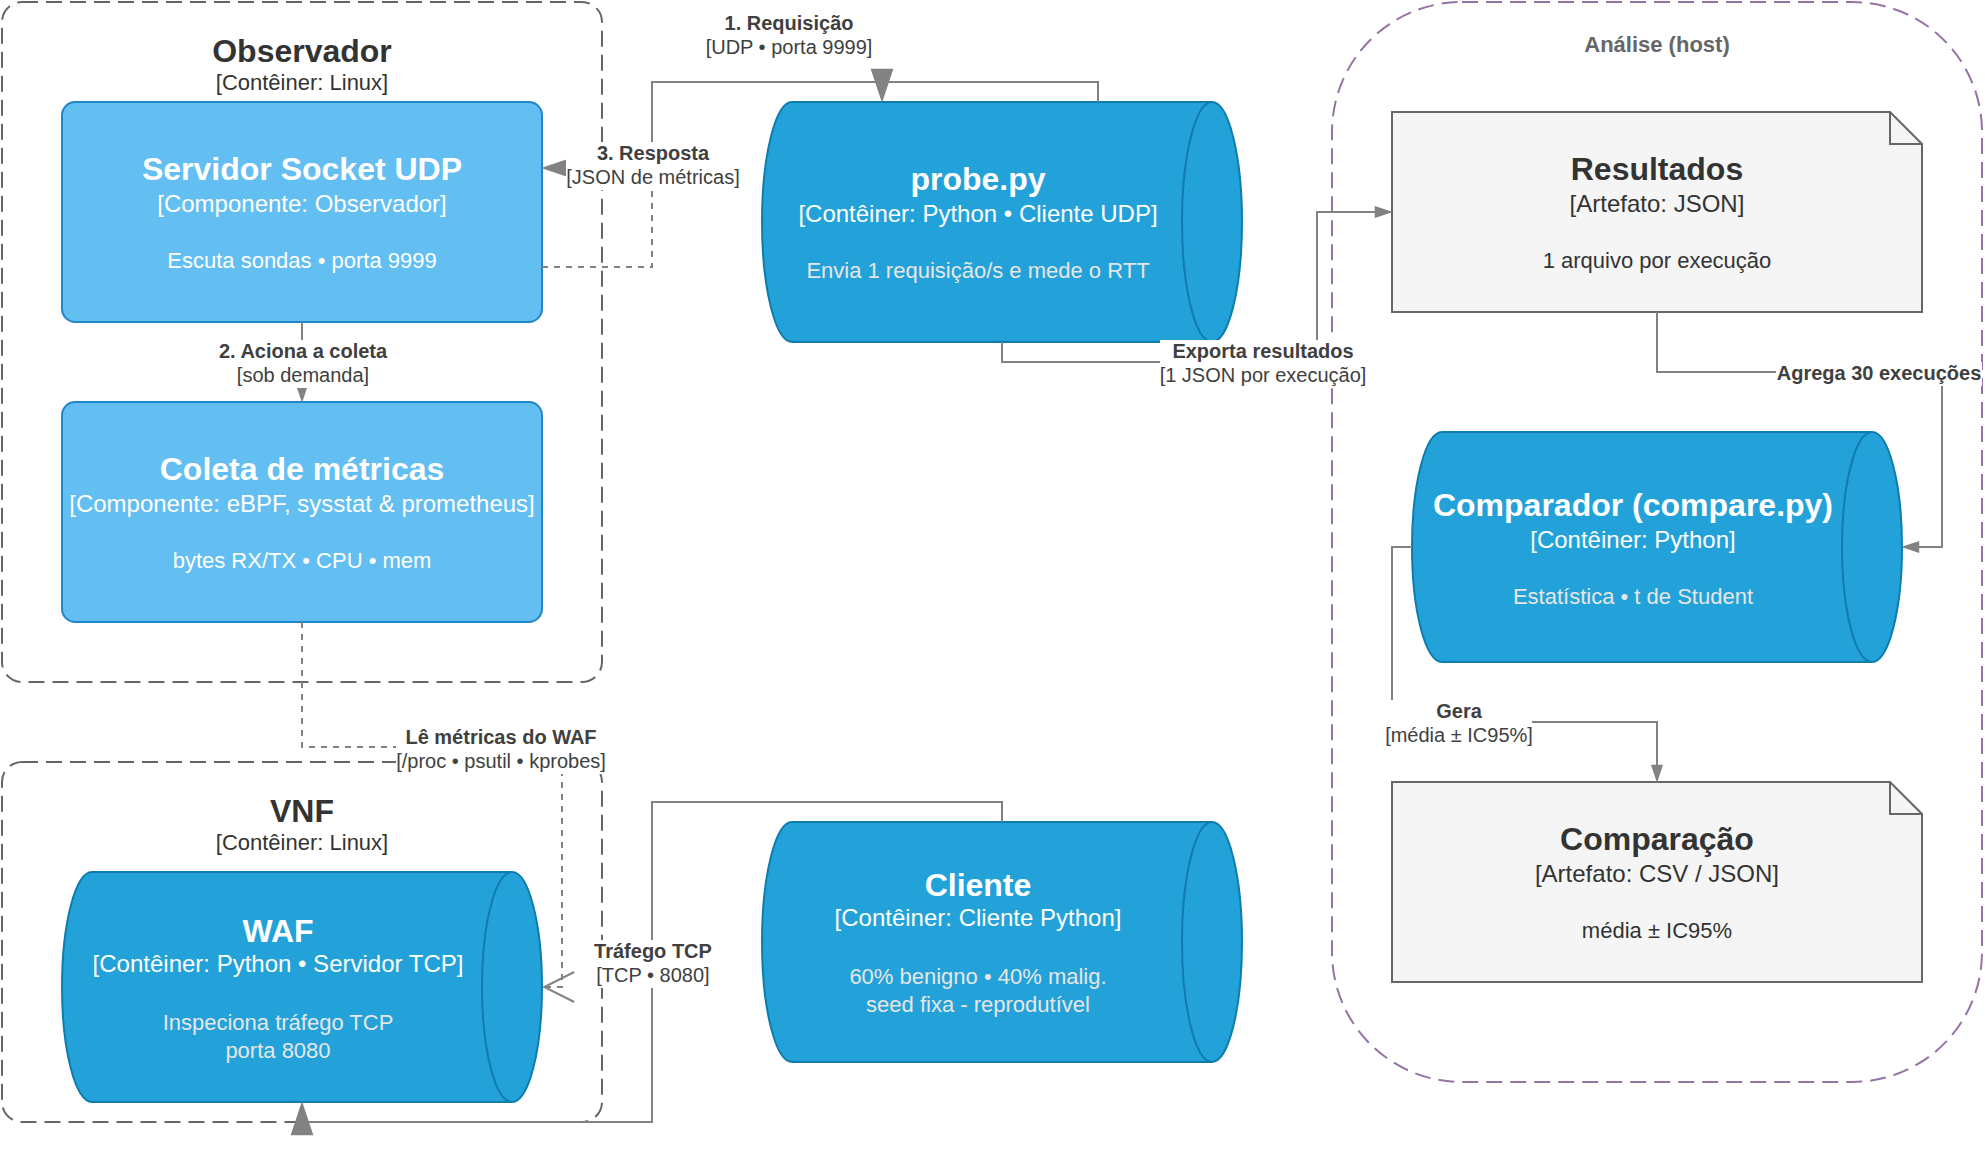
\includegraphics[width=0.85\textwidth]{imagens/C4model.drawio.png}
    \caption{Diagrama de contêineres (C4, Nível 2) da topologia experimental.}
    \label{fig:arquitetura_c4}
\end{figure}

O processo de medição é realizado pelo \texttt{probe.py}, que envia uma requisição UDP a cada 1 segundo para o observador ativo. O tempo de ida e volta é medido com resolução de nanossegundos via \texttt{time.time\_ns()}, sendo esta a métrica primária de sobrecarga do monitoramento. Antes de iniciar a coleta, o \texttt{probe.py} aguarda até 60 segundos pela disponibilidade do observador, garantindo que nenhuma amostra seja registrada antes da inicialização completa do coletor.

\section{Implementação dos Coletores}

\subsection{Coletor eBPF}

O coletor eBPF utiliza a biblioteca \textit{libbpf} com a abordagem CO-RE, que elimina a dependência do arcabouço BCC/LLVM em tempo de execução e permite que o programa BPF compilado seja portável entre versões de kernel compatíveis \cite{gregg_bpf_2019}. O programa em C (\texttt{ebpf\_kern.c}) é compilado para \textit{bytecode} eBPF durante a construção da imagem Docker e carregado no kernel na inicialização do observador.

Dois programas são anexados por meio de \textit{kprobes}: (a) \texttt{kprobe/tcp\_sendmsg}: intercepta cada chamada de envio TCP, acumulando os bytes transmitidos (TX) para conexões cuja porta de origem é 8080; e (b) \texttt{kprobe/tcp\_cleanup\_rbuf}: intercepta a liberação do \textit{buffer} de recepção TCP, acumulando os bytes recebidos (RX) para a mesma porta. Os contadores são armazenados em mapas eBPF do tipo \texttt{HASH}, chaveados pelo identificador da conexão. O processo em espaço do usuário lê esses contadores de forma assíncrona a cada solicitação recebida, sem cópias de pacotes e sem pressão adicional sobre a pilha de rede.

\subsection{Coletor Sysstat}

O coletor Sysstat opera de forma reativa: a cada requisição UDP recebida, lê o arquivo \texttt{/proc/net/dev} e extrai os contadores acumulados de bytes RX e TX da interface de loopback (\texttt{lo}), calculando o delta em relação ao valor inicial para estimar o tráfego acumulado desde o início do experimento \cite{godard2024sysstat}. O consumo de CPU e de memória do processo WAF é obtido pela biblioteca \texttt{psutil}, que consulta os arquivos \texttt{/proc/<pid>/stat} e \texttt{/proc/<pid>/status}.

\subsection{Coletor Prometheus}

% CORREÇÃO overflow: /proc/net/dev quebrado com \linebreak[0]
O coletor Prometheus adota a mesma lógica de coleta do Sysstat (leitura de \texttt{/proc/\linebreak[0]net/dev} e \texttt{psutil}), com o acréscimo de um servidor HTTP na porta 8000, implementado com a biblioteca \texttt{prometheus\_client} do Python \cite{turnbull_prometheus_2018}. Esse servidor expõe as métricas coletadas no formato padrão Prometheus via \texttt{/metrics}, habilitando a integração com um servidor de coleta externo. Neste experimento, nenhum servidor Prometheus externo realiza a coleta das métricas: o \textit{endpoint} permanece disponível, mas não é consultado durante os testes, o que restringe o escopo à sobrecarga do processo exporter em si, excluindo o custo do ciclo completo de \textit{scraping} presente em implantações reais. A sobrecarga adicional em relação ao Sysstat decorre exclusivamente da presença do servidor HTTP em execução, que consome ciclos de CPU para manter o \textit{socket} aberto e serializar as métricas a cada atualização interna.

O código-fonte dos três coletores, da geração de carga e da análise estatística está disponível publicamente no GitHub\footnote{https://github.com/joaopedroplinta/vnf-monitoring-benchmark}.

\section{Protocolo de Testes e Geração de Carga}

Neste experimento, o volume de mensagens N constitui a variável independente, assumindo quatro níveis: 100.000, 500.000, 1.000.000 e 2.000.000. A variável dependente primária é o tempo de resposta do observador (RTT UDP); CPU e memória do WAF e do coletor são variáveis dependentes secundárias, utilizadas para caracterizar a sobrecarga de cada abordagem.

As cargas são geradas previamente pelo script \texttt{gen\_payloads.py}, que produz arquivos binários com N mensagens nos quatro volumes citados. Cada arquivo contém 60\% de cargas benignas (textos aleatórios com caracteres ASCII imprimíveis) e 40\% de cargas maliciosas, intercaladas aleatoriamente com semente fixa \texttt{42} (\texttt{--seed 42}), garantindo que a sequência de mensagens seja idêntica entre ferramentas e volumes, condição necessária para a validade comparativa do experimento. O cliente lê as cargas sob demanda via fila assíncrona, mantendo o consumo de memória constante independentemente do volume N. A duração de cada execução é calculada de acordo com a Equação \ref{eq:duration}:

\begin{equation}
\text{DURATION} = \lfloor N / 15000 \rfloor + 20 \text{ segundos}
\label{eq:duration}
\end{equation}

O divisor 15.000 corresponde à taxa de vazão sustentada empiricamente pelas 200 corrotinas assíncronas no ambiente de testes, expressa em mensagens por segundo; os 20 segundos adicionais constituem uma margem de segurança para a inicialização e o encerramento dos contêineres. Esse valor garante que o cliente complete o envio de todas as cargas e que o observador capture amostras suficientes para a análise. Para cada combinação de coletor e volume N, foram realizadas \textbf{30 repetições} independentes, totalizando 360 execuções (3 coletores $\times$ 4 volumes $\times$ 30 repetições). Cada repetição executa o ciclo completo: inicialização dos contêineres, aquecimento do observador, coleta de dados e encerramento controlado via \texttt{docker compose down}.

Em cinco das 360 execuções, verificou-se \texttt{inspect\_count = 0} e \texttt{inspect\_avg\_ms = 0}, causados por uma condição de execução na leitura do arquivo \texttt{waf\_metrics.json}: o \texttt{probe.py} encerrou a coleta antes de o WAF gravar o arquivo pela primeira vez naquela execução. O critério adotado foi o seguinte: como a condição de execução afeta exclusivamente a leitura do arquivo \texttt{waf\_metrics.json} e não o mecanismo de requisição UDP, as medições de tempo de resposta UDP dessas execuções são válidas e estão incluídas nas agregações da métrica primária, preservando o tamanho amostral de 30 repetições para essa métrica; as métricas de inspeção (\texttt{inspect\_count}, \texttt{inspect\_avg\_ms}, \texttt{inspect\_min\_ms}, \texttt{inspect\_max\_ms}) dessas cinco execuções, cujos valores são zero por definição e não refletem o comportamento real do WAF, são desconsideradas nas análises de inspeção do WAF para não distorcer as médias.

\section{Métricas Coletadas e Análise Estatística}

O \texttt{probe.py} registra, a cada requisição, as seguintes métricas \cite{rfc8172}:

\begin{itemize}
    \item \textbf{Tempo de resposta do observador} (\texttt{observador\_latency\_avg\_ms}): tempo de ida e volta da requisição UDP em milissegundos, constituindo a métrica primária de sobrecarga do monitoramento;
    \item \textbf{CPU do WAF} (\texttt{cpu\_avg\_pct}): consumo médio de CPU do processo WAF durante o experimento;
    \item \textbf{Memória do WAF} (\texttt{mem\_avg\_mb}): consumo médio de memória RSS do processo WAF;
    \item \textbf{CPU do observador} (\texttt{collector\_cpu\_avg\_pct}): consumo médio de CPU do próprio observador;
    \item \textbf{Memória do observador} (\texttt{collector\_mem\_avg\_mb}): consumo médio de memória RSS do observador;
    \item \textbf{Bytes RX/TX} (\texttt{bytes\_rx}, \texttt{bytes\_tx}): volume acumulado de bytes recebidos e transmitidos. Não são diretamente comparáveis entre as ferramentas, pois o coletor eBPF contabiliza apenas o tráfego do WAF (filtrando \texttt{sport = 8080} no \textit{kernel}), enquanto o Sysstat e o Prometheus medem todo o tráfego da interface de \textit{loopback};
    % CORREÇÃO overflow: \raggedright local no item com os três \texttt longos
    \item {\raggedright\textbf{Métricas de inspeção do WAF}: contagem total de inspeções (\texttt{inspect\_count}), tempo médio, mínimo e máximo por inspeção (\texttt{inspect\_avg\_ms}, \texttt{inspect\_min\_ms}, \texttt{inspect\_max\_ms}).\par}
\end{itemize}

Destas, as cinco primeiras (tempo de resposta, CPU e memória do WAF e do observador) constituem as \textbf{métricas de comparação} entre as abordagens, conforme a discussão da Seção~\ref{subsec:requisitos_monitoramento}. As duas últimas (bytes RX/TX e métricas de inspeção) são \textbf{métricas de validação e caracterização}: confirmam que as três ferramentas processaram a mesma carga e caracterizam o custo de inspeção do WAF, mas não compõem a comparação entre coletores --- seja por independerem do coletor empregado (tempo de inspeção), seja por não serem mutuamente comparáveis (bytes RX/TX).

Os resultados das 30 repetições são agregados pelo script \texttt{compare.py}, que calcula a \textbf{média aritmética} e o \textbf{intervalo de confiança de 95\%} (IC95\%) para cada métrica, utilizando a distribuição t de Student \cite{marconi2017}. O IC95\% é calculado pela Equação \ref{eq:ic95}.

\begin{equation}
\text{IC}_{95\%} = t_{(n-1;\;0{,}025)} \cdot \frac{s}{\sqrt{n}}
\label{eq:ic95}
\end{equation}

\noindent onde $n = 30$ é o número de repetições, $s$ é o desvio padrão amostral entre as repetições e $t_{(29;\;0{,}025)} = 2{,}045$ é o quantil da distribuição t de Student bicaudal com $n - 1 = 29$ graus de liberdade e nível de significância $\alpha = 0{,}05$. Os resultados são apresentados no formato $\bar{x} \pm \text{IC}_{95\%}$, onde $\bar{x}$ é a média das 30 repetições. Os resultados finais são exportados nos formatos CSV e JSON para análise comparativa entre as três ferramentas.

Reconhecem-se as seguintes limitações dos experimentos: (i) o tráfego que flui pela interface de loopback (\texttt{lo}), o que elimina o overhead de drivers de NIC físico presentes em ambientes de produção; isso implica que os valores absolutos de latência UDP e de bytes RX/TX são inferiores ao que se observaria em uma rede física, onde interrupções de hardware e transferências DMA adicionam carga à CPU e aumentam a variância das medições; (ii) todos os contêineres compartilham o mesmo kernel e núcleos de CPU, de modo que contenção de recursos entre cliente, WAF e observador é possível; (iii) o WAF é uma implementação simplificada em Python, cujo perfil de CPU difere de soluções de produção como o ModSecurity. Contudo, por ser idêntico em todos os experimentos, garante que as diferenças observadas entre os coletores reflitam exclusivamente o custo de cada abordagem de monitoramento, e não características da VNF em si. Esses fatores limitam a generalização direta dos resultados absolutos, sem prejuízo à validade comparativa entre as três abordagens avaliadas sob as mesmas condições.
